% Dmitry Mikushin, USI Lugano, dmitry.mikushin@usi.ch,
% using portions of original style file by Tom Cashman
%
% IMPORTANT NOTICE:
%
% The USI logo is unique; it is authorized for use only by employees of the
% Università della Svizzera italiana for work-related projects; others can use them
% ONLY with prior authorization (contact: press@usi.ch).
%
% http://www.press.usi.ch/en/corporate-design/corporate-design-stampa.htm
%
% This is an example beamer presentation, which uses Università della Svizzera italiana
% design theme.

\documentclass[aspectratio=169]{beamer}

\usetheme{usi}

\usepackage{comment}
\usepackage{tikz}
\usepackage{listingsutf8}
\usepackage{xcolor}
\usepackage{beramono}
\usepackage{polyglossia}

\defaultfontfeatures{Scale=MatchLowercase, Mapping=tex-text}

\usetikzlibrary{shapes,arrows}
\usetikzlibrary{shadows}

\setmainfont{Trebuchet MS}
\setsansfont{Trebuchet MS}
%\setmonofont{Courier New}

% Draw frame around picture
\setlength{\fboxsep}{0pt}%
\setlength{\fboxrule}{0.25pt}%

\title[Coffee with science and milk -- USI 10 Years Anniversary Activities]{Coffee with science and milk}
\subtitle{USI 10 Years Anniversary Activities}
\author{Dmitry Mikushin}
\institute{}
\date{\today}

\begin{document}

\begin{frame}
\titlepage
\end{frame}



\begin{frame}[fragile]{The demonstration}

\underline{Purpose:} introduce general audience into fluid\\ dynamics by example of e.g. mixing coffee with spoon.

\vskip10pt

A non-reactive substance injected into the fluid:

\begin{itemize}
\item Coffee and milk
\item Steam or smoke
\item ...
\end{itemize}

\begin{tikzpicture}[remember picture,overlay]
  \node [xshift=12cm,yshift=-4.20cm] at (current page.north west){%
    \fbox{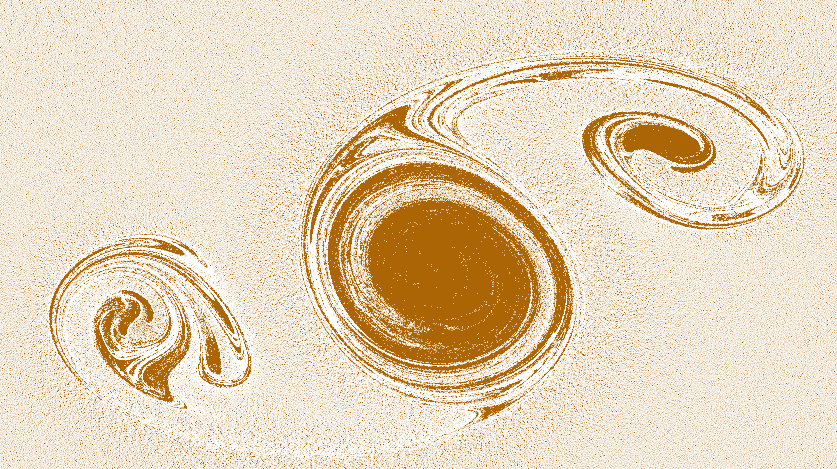
\includegraphics[height=3.5cm]{figures/whirl}}};
\end{tikzpicture}

\end{frame}



\begin{frame}[fragile]{The booth}

\begin{center}
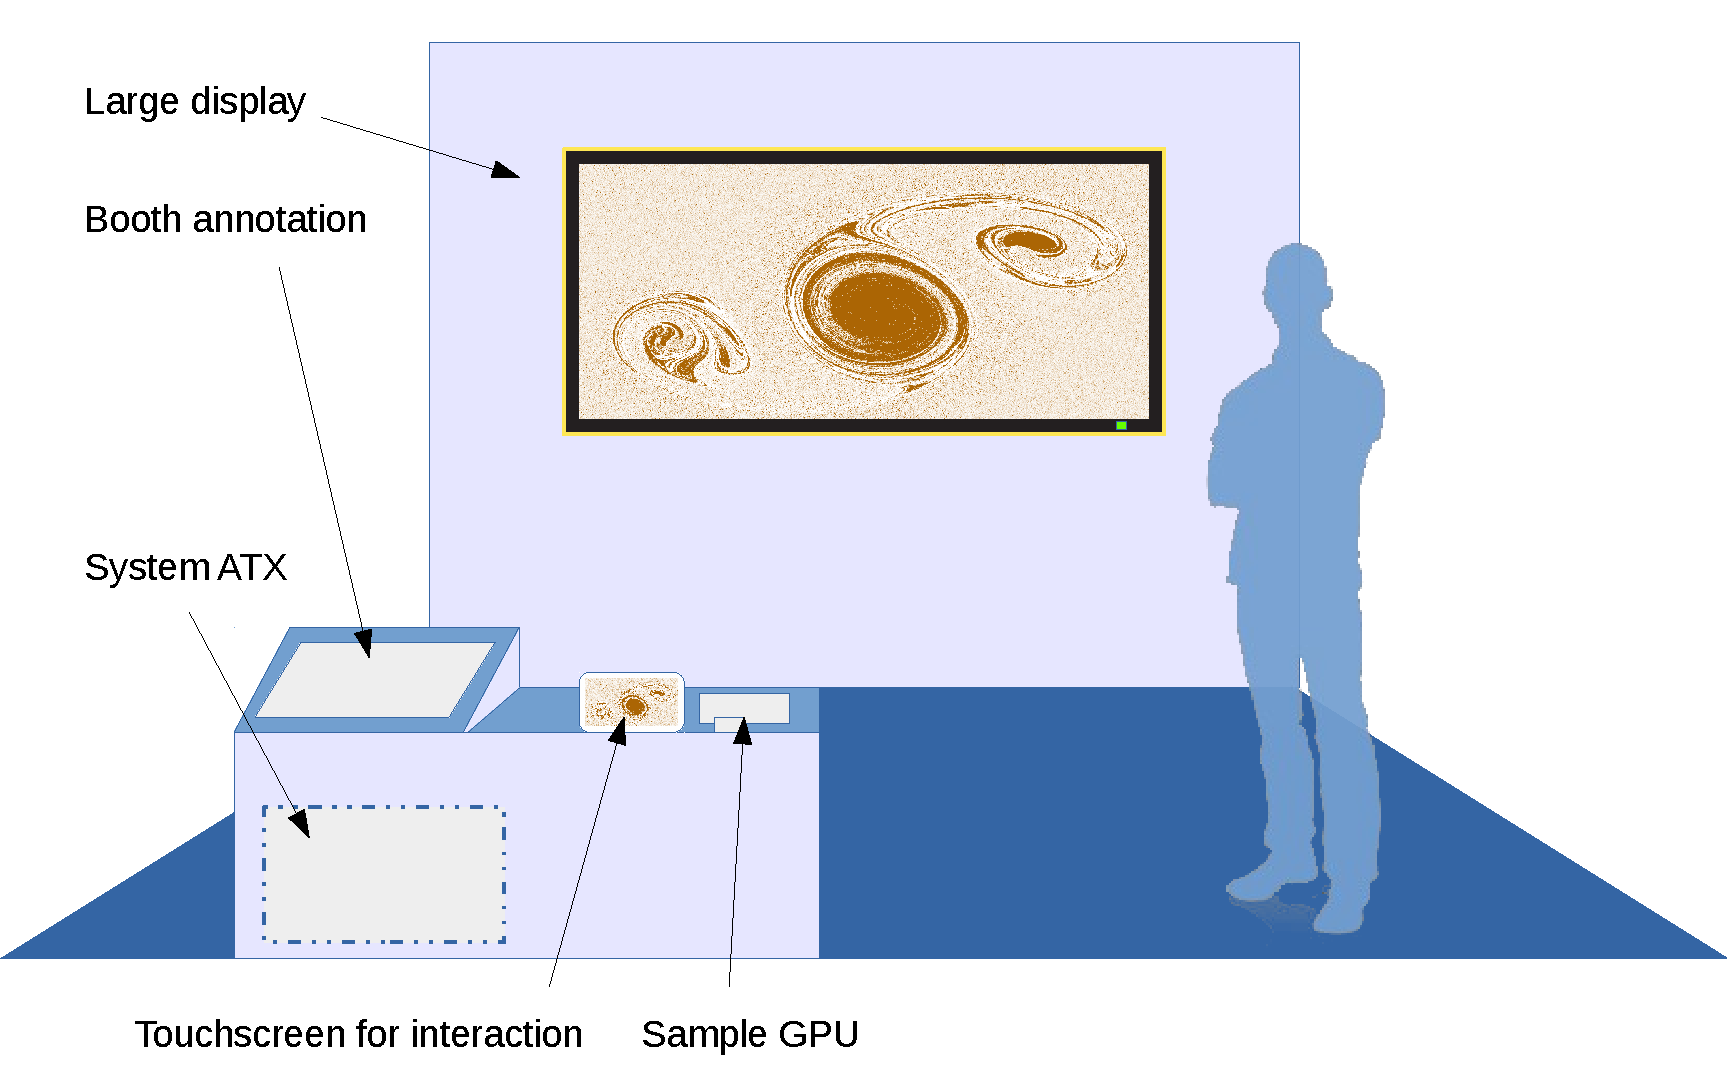
\includegraphics[width=11cm]{figures/booth}
\end{center}

\end{frame}



\begin{frame}[fragile]{Numerical background}

\begin{itemize}
\item Navier-Stokes for 2D incompressible fluid, with periodic BC:
\vskip5pt
\begin{itemize}
\item[-] Advection: method of characteristics
\item[-] Diffusion \& projection: FFT, implicit scheme for diffusion
\item[-] Passive particles transfer
\end{itemize}
\end{itemize}
\vskip10pt
For more details please refer to the paper:
\vskip8pt
Stam, J. 1999. ``Stable Fluids.'' In Proceedings of SIGGRAPH 1999. \href{http://www.dgp.toronto.edu/people/stam/reality/Research/pdf/ns.pdf}{http://www.dgp.toronto.edu/people/stam/reality/Research/pdf/ns.pdf}
\end{frame}



\begin{frame}[fragile]{Computational background}

\begin{itemize}
\item GPU implementation -- Sample \emph{fluidsGL} -- a part of CUDA SDK since 2009
\vskip5pt
\begin{itemize}
\item[-] CUDA simulation + OpenGL visualization
\item[-] CUDA \& OpenGL on the same GPU or on different -- for Optimus\\ (large FPS loss due to host-gpu data transfers, see profile figure)
\item[-] Up to 35 FPS on GTX 680M  with Optimus, 2048$\times$2048
\end{itemize}
\end{itemize}

\vskip5pt

\hskip43pt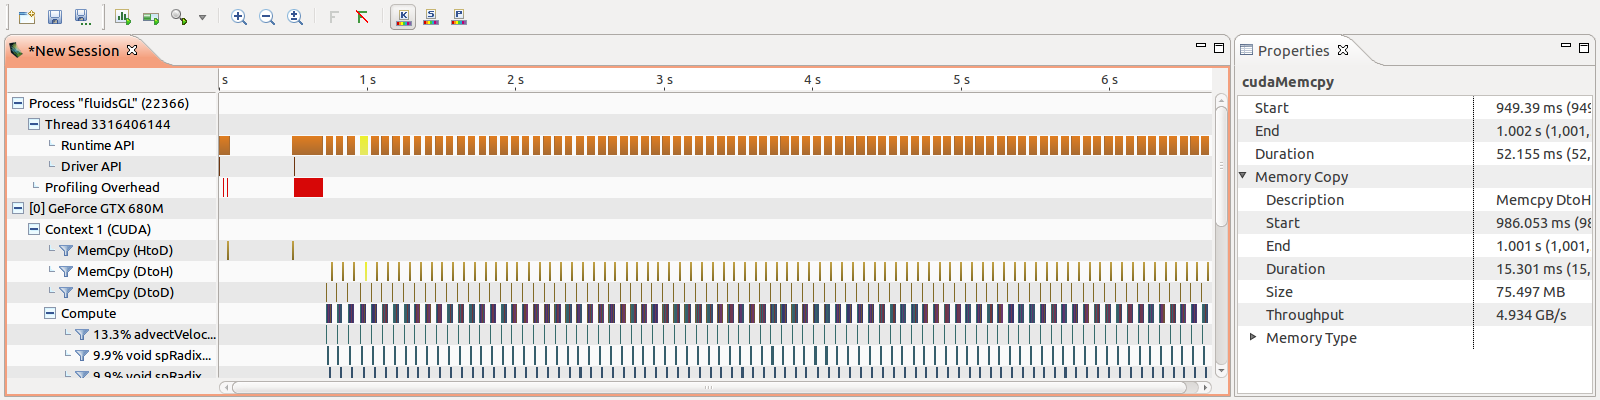
\includegraphics[width=12cm]{figures/profiler}

\end{frame}



\begin{frame}[fragile]{Testing \& development}

Current source code available here: \href{https://github.com/dmikushin/fluidsGL-optimus}{https://github.com/dmikushin/fluidsGL-optimus}

\end{frame}

\end{document}
